%\newcommand{\nl}{$n_{\ell}$ }
\newcommand{\km}{\textless k \textgreater}
\chapter{Structure des réseaux sans échelle non corrélés: couches et plus court chemin}
\label{sec3}
\begin{minipage}{\textwidth}
	\linespread{1.2}
	\minitoc
\end{minipage}

\section{Introduction}
L'objectif principal de ce chapitre vise à prédire la structure des couches
des réseaux sans échelles en nous basant sur les propriétés locales régissant les sommets individuels.\\
De nombreux réseaux du monde réel qui ont été décrits précédemment, tels que le WWW et les réseaux de collaboration, grandissent avec le temps. Par conséquent, il est raisonnable de considérer les graphes de taille croissante et d'étudier la structure de ces réseaux ayant souvent la propriété sans échelle (voir Section.\ref{s-libre-echelle}). 
La communauté scientifique, en s'appuyant sur des idées issues d'une grande variété de disciplines, a fait un excellent départ sur la caractérisation et la modélisation de la structure des réseaux, mais il n'y pas encore de formalisme théorique bien établi \cite{Ne2003}. Dans ce chapitre nous allons expliquer notre contribution à la compréhension de la structure intrinsèque des réseaux sans échelle. En particulier, nous allons calculer le nombre moyen de voisins d'un nœud  donné se trouvant à une distance précise, et nous allons en déduire le plus court chemin dans le réseau.% Nous allons commencer par quelques propriétés et définitions, et ensuite on va rappeler quelques travaux importants dans le sujet. Dans la dernière section du chapitre nous exposons nos calculs  détaillés.
\section{Caractérisation des réseaux sans échelle}
Un réseau sans échelle (ou réseau invariant d'échelle, ou encore scale-free network en anglais) est un réseau dont la distribution des degrés suit une loi de puissance, c'est-à-dire, $P(k)=Ck^{-\gamma}$, où $C$ est une constante.  Donc, dans un tel réseau, la proportion de nœuds de degré $k$ est proportionnelle à $k^{-\gamma}$. Cette loi traduit l'absence d'échelle caractéristique. En effet, si on multiplie $k$ par une constance $\alpha$, $P(\alpha k)=C\alpha^{-\gamma}k^{-\gamma}=C' k^{-\gamma}$, donc les propriétés sont les mêmes si on change l'échelle.\\ 
Identifier la loi de puissance dans les systèmes naturels ou artificiels peut être difficile. La stratégie standard utilise le fait que la courbe d'une distribution sans échelle apparaît comme une ligne droite lorsqu'elle est tracée sur des échelles logarithmiques (voir Fig.~\ref{sans-echelle-3}).
\begin{figure}[h!]
	\centering
	\includegraphics[scale=1.2]{./figures/fig-sans-echelle}
	\caption{Illustration de la loi de puissance pour une fonction, $P(k)=k^{-\gamma}$, avec l'exposant $\gamma=3$. Dans a) l'échelle est logarithmique et dans b) l'échelle est linéaire.}
	\label{sans-echelle-3}
\end{figure}
Cependant, la méthode n'est pas très bonne à certains égards. En particulier, l'extrémité de la droite de la distribution est bruyante en raison d'erreurs d'échantillonnage (voir Fig.~\ref{BA-distribution}). Du fait que la distribution diminue dans l'extrémité,  chaque valeur mesurée ne contient que quelques échantillons, et les fluctuations dans les valeurs mesurées sont grandes, et cela apparaît comme une courbe bruyante sur la figure. Une façon de traiter cela est de simplement jeter les données dans la queue de la courbe. Mais il y a souvent des informations utiles dans ces données, car de nombreuses distributions suivent une loi de puissance seulement dans la queue. Une solution alternative consiste à faire varier la largeur des cases dans notre courbe. Le nombre d'échantillons dans une largeur $\Delta x$ devrait être divisé par $\Delta x$ pour obtenir une moyenne par intervalle unitaire de $x$. Ensuite, le nombre d'échantillons normalisé devient indépendant de la largeur de la valeur mesurée en moyenne, et nous sommes libres de varier les largeurs $\Delta x$ comme nous le souhaitons. Le choix le plus commun est de créer des largeurs telles que chacune est un multiple fixe plus large que celui qui le précède, ce qui est connu sous le nom "logarithmic binning". Ceci réduit les erreurs statistiques dans la queue. En outre, les valeurs mesurées semblent être de largeur constante quand nous traçons la courbe sur des échelles logarithmiques.
\section{Quelques notions mathématiques de la loi de puissance}
Une variable réelle continue avec une distribution en loi de puissance a une probabilité $P(k)$ de prendre une valeur $k$, où
\begin{equation}
P(k)=Ck^{-\gamma}.
\label{3-1}
\end{equation}
Comme nous avons vu dans la Section.~\ref{s-libre-echelle}, l'exposant $\gamma$ et la variable $k$ sont positifs. \\
Dans les réseaux réels, les distributions de degrés ne suivent généralement pas une loi de puissance pure sur toute leur gamme.
En regardant la Fig.~\ref{scal-free-reels}, par exemple, nous observons que la distribution de degrés n'est pas toujours monotone pour les petits $k$, même en tenant compte des fluctuations statistiques dans l'histogramme. Quand on dit qu'un réseau a une distribution de degré sans échelle, on se réfère implicitement à la queue de la distribution, qui doit avoir cette forme. Cependant, et dans certains cas, la distribution peut  s'écarter de la loi d'échelle pour $k$ élevé. En fait, il y a parfois une coupure qui limite le degré maximum de nœuds dans la queue.\\
La constante $C$ dans l'Eq.~\eqref{3-1} est la constante de normalisation qui s'obtient en intégrant:
\begin{equation}
P(k)=\int_m^{\infty}Ck^{-\gamma}dk=1,
\label{3-2}
\end{equation}
où $m$ est le degré minimum dans le réseau, on obtient
\begin{equation}
C=(\gamma-1)m^{\gamma-1},
\end{equation}
alors l'Eq.~\eqref{3-1} devient:
\begin{equation}
P(k)=(\gamma-1)m^{\gamma-1}k^{-\gamma}.
\label{3-4}
\end{equation}
%\subsection{Moments}
Le $j^{\text{ème}}$ moment de la distribution $P(k)$ est défini comme:
\begin{align}
\textless k^j\textgreater&=\int_{m}^{\infty} k^jP(k)dk\nonumber\\
&=(\gamma-1)m^{\gamma-1}\int_{m}^{\infty}k^{j-\gamma}dk.
\end{align}
Le premier moment $\textless k\textgreater$  est le degré moyen de $k$, notons que $\textless k\textgreater$  devient infini si $\gamma\leq2$. Le second moment $\textless k^2\textgreater$ mesure les fluctuations de $k$, il diverge si $\gamma\leq3$. Sachant que dans les réseaux réels l'exposant $\gamma$ est souvent dans l'intervalle $2<\gamma<3$, ceci implique que les fluctuations divergent dans ces réseaux.\\
%\subsection{Loi sans échelle pour les variables discrètes
En réalité, dans un réseau, les degrés sont des entiers naturels, et dans nos calculs les intégrales doivent être remplacées par des sommes. Mais, puisque la loi d'échelle
n'est vérifiée que pour les grands degrés, ceux-ci peuvent être considérés comme représentant  une variable continue.\\
Techniquement, si $k$ est une variable discrète, et $P(k)=Ck^{-\gamma}$, alors la constante de normalisation $C$ doit vérifier $\sum_{k=1}^{\infty}Ck^{-\gamma}=1$, donc $C=\frac{1}{\zeta(\gamma)}$, et $\zeta(\gamma)$ est la fonction zêta de Riemann. Donc la loi de puissance, si $k$ est discret, s'écrit:
\begin{equation}
P(k)=\frac{1}{\zeta(\gamma)}k^{-\gamma}.
\label{pk-descret}
\end{equation}
Dans les calculs on a souvent besoin de connaître la valeur du degré maximum $K$, mais dans un réseau dans échelle en croissance, ce n'est pas possible de connaître sa valeur exacte. Pour estimer la valeur de $K$, on suppose que dans un réseau fini avec $n$ nœud , on peut avoir au plus un nœud dans l'intervalle $[K,\infty[$, c'est-à-dire, la probabilité d'observer un nœud avec un degré supérieur à $K$ est $\frac{1}{n}$, donc:
\begin{equation}
\int_{K}^{\infty}P(k)dk=\frac{1}{n},
\end{equation}
d'où on obtient $K= mn^{\frac{1}{\gamma-1}}$.
\section{Les réseaux sans échelle non corrélés}
Dans les modèles aléatoires sans échelle, on suppose généralement qu'il n'y a pas de corrélation entre les degrés des nœuds voisins. C'est-à-dire que la probabilité d'atteindre un nœud en suivant un lien est indépendante du nœud d'où provient le lien. Cependant, dans de nombreux réseaux du monde réel, ce n'est pas le cas. Plusieurs types de corrélations existent en fonction des propriétés des nœuds. Les principaux types de corrélations étudiées sont les corrélations degré-degré (voir Section.\ref{s-correl}). Même si la construction de ces réseaux sans échelle aléatoires se fait au départ sans aucune corrélation, cela ne signifie pas que le réseau n'affichera pas des corrélations de degré, c'est-à-dire l'absence de corrélations lors de la création des réseaux n'entraîne pas l'absence de corrélations dans le réseau formé.  La Fig.~\ref{correlation} indique que les réseaux aléatoires sans échelle présentent des corrélations de degré, allant de l'assortativité à la dissassortativité selon la valeur de l'exposant $\gamma$. Nous observons trois situations:
%\begin{spacing}{1.5}
\begin{itemize}
	\item[i)] $\gamma>3$, le réseau est dit assortatif. Dans ce cas, la corrélation entre les degrés des sommets et ceux de leurs voisins est élevée. Autrement dit, les sommets ayant un degré élevé sont connectés entre eux; les sommets ayant un degré faible sont connectés entre eux et il y a peu de liens entre les sommets de degré élevé et ceux de degré faible 
	\item[ii)]$\gamma=3$, le réseau est neutre.
	\item[iii)]$\gamma<3$, le réseau est dissassortatif. C'est le cas contraire à l'assortativité. Les sommets voisins sont peu corrélés, et les sommets avec un degré élevé sont connectés à ceux avec un degré faible.  
\end{itemize}
%\end{spacing}
Générer des corrélations en utilisant un modèle complètement statique est difficile car non seulement le degré d'un nœud doit être pris en compte, mais aussi sa probabilité de se connecter à chaque voisin. La méthode habituellement utilisée pour générer ces réseaux corrélés consiste à mélanger les liens en utilisant une sorte d'algorithme de type Metropolis\footnote{Inventé en 1953 par Nicholas Metropolis et ses collaborateurs du laboratoire de Los Alamos, l'algorithme de Metropolis était d'abord destiné à faire calculer par des ordinateurs les équations d'états de mélanges de molécules en interactions. L'outil principal de l'algorithme est une chaîne de Markov : on tire au hasard une boule et on déplace son centre d'une distance $d$, le mouvement est accepté si la nouvelle configuration des boules reste sans recouvrement.} \cite{Metropolis-al1953}.\\ Cependant, la négligence de ces corrélations n'empêche jamais de trouver des résultats importants, qui nous aideront à bien modéliser ces réseaux réels et à mieux comprendre leurs structures. 
\begin{figure}[h!]
	\centering
	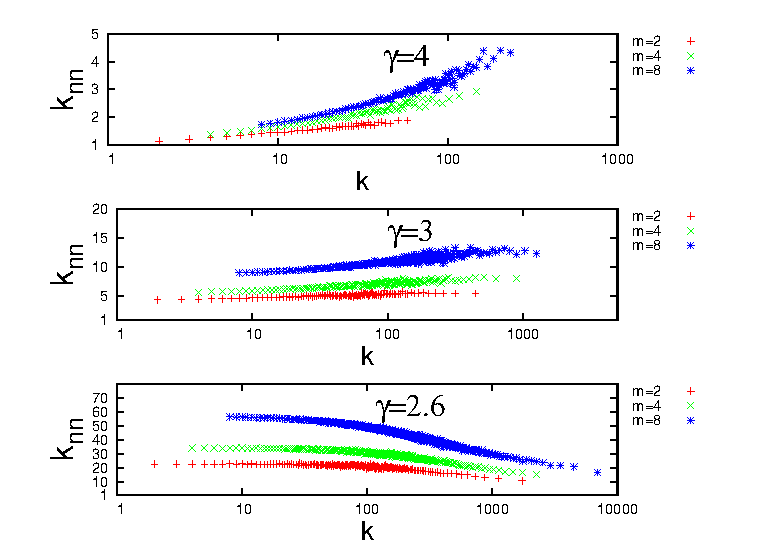
\includegraphics[scale=1.2]{./figures/correlation}
	\caption{Les corrélations des degrés dans le réseau aléatoire sans échelle pour différents valeurs de $m$ et de $\gamma$. Le nombre de nœuds est $n=10^4$ et le nombre de réalisations pour chaque simulation est $50$.}
	\label{correlation}
\end{figure}
\vspace{3cm}
\section{Structure des couches dans les réseaux sans échelle non corrélés}
\subsection{Quelques contributions importantes}
Newman est l'un des premiers à chercher une expression explicite pour les couches dans les réseaux complexes \cite{Newman2010-456}, où le mot couche désigne le nombre moyen de nœuds à une distance donnée d'un nœud arbitraire choisi au hasard, et qu'on appelle nœud racine.\\
Le calcul de Newman se base sur la fonction génératrice qui suscite un intérêt particulier dans les réseaux complexes. En effet, celle-ci donne toute l'information sur la distribution des degrés $P(k)$. La fonction génératrice est le polynôme:
\begin{equation}
g(z)=P(0)+P(1)z+P(2)z^2+...=\sum_{k=0}^{\infty}P(k)z^k.
\end{equation}
Si on connaît la fonction génératrice, on peut récupérer les valeurs de $P(k)$ en différenciant:
\begin{equation}
P(k)=\frac{1}{k!}\frac{d^kg(z)}{dz^k}\Big\lvert_{z=0}.
\end{equation}
Ainsi, la distribution de probabilité et la fonction génératrice ne sont en réalité que deux représentations différentes de la même chose. Dans de nombreux cas, il est plus facile de travailler avec la fonction génératrice qu'avec la distribution de probabilité.\\
Soit $p_k^{(2)}$ la probabilité qu'un nœud a exactement $k$ seconds voisins dans le réseau
\begin{equation}
p_k^{(2)}=\sum_{s=0}^{\infty}P(s)P^{(2)}(k/s),
\end{equation}
avec $P^{(2)}(k/s)$ la probabilité d'avoir $k$ seconds voisins étant donné que nous avons $s$ premiers voisins, et $P(s)$ est la distribution de degrés.\\
La fonction génératrice de cette probabilité s'écrit:

\begin{align}
	g^{(2)}(z)&=\sum_{k=0}^{\infty}p_k^{(2)}z^{k}\nonumber\\
	%&=\sum_{m=0}^{\infty}p_m\sum_{k=0}^{\infty}P^{(2)}(k/m)z^k\nonumber\\
	%&=\sum_{m=0}^{\infty}p_m[g_1(z)]^m\nonumber\\
	&=g_0(g_1(z)),
	\label{p-generatrice-2}
\end{align}
avec $g_0(z)=\sum_{k=0}^{\infty}P(k)z^k$ et $g_1(z)=\frac{1}{g'_0(1)}\frac{dg_0}{dz}$, (nous utiliserons la notation $g'$, car elle s'avère beaucoup moins lourde que la notation plus courante $\frac{dg}{dz}$.).\\
En généralisant la procédure, Newman a trouvé la fonction génératrice du nombre de voisins à n'importe quelle distance $\ell$, qui s'écrit:
\begin{align}
g^{(\ell)}(z)&=\sum_{s=0}^{\infty}p_s^{(\ell-1)}\sum_{k=0}^{\infty}P^{(\ell)}(k/s)z^k\\
&=g^{(\ell-1)}(g_1(z)),
\label{p-generatrice-l}
\end{align}
avec $g^{(\ell)}(z)=g_0(...g_1(z)...)$, où dans $g_0$ il y a $\ell-1$ copie de $g_1$.\\
Il est généralement difficile d'extraire les expressions explicites des probabilités à partir de l'équation précédente, et ce m\^{e}me pour le cas des seconds voisins. Cependant, pour une distribution de degrés suivant la loi de Poisson avec une moyenne $\km$, $P(k)=\frac{\km^k}{k!}e^{-\km}$, et si on suppose que $z=1$, le calcul se simplifie pour le nombre de seconds voisins, et on trouve:
\begin{equation}
n_2=g_0'(1)g_1'(1),
\label{3-27}
\end{equation}
sachant que $g_0'(1)=\km$ et $g_1'(1)=\frac{1}{\km}(\textless k^2\textgreater-\km)$, on obtient
\begin{equation}
n_2=\textless k^2\textgreater-\km.
\end{equation}
Le nombre moyen de voisins $n_{\ell}$ à n'importe quelle distance $\ell$, pour une distribution de poisson, est obtenu à partir de l'Eq.~\eqref{p-generatrice-l}:
\begin{equation}
\frac{dg^{(\ell)}}{dz}=g^{(\ell-1)'}(g_1(z))g_1'(z),
\end{equation}
sachant que nous avons choisi $z=1$ nous pouvons écrire 
\begin{align}
n_{\ell}&=g^{(\ell-1)'}(1)g_1'(1)\\
&=n_{\ell-1}g_1'(1),\nonumber
\end{align}
de l'Eq.~\eqref{3-27}, et sachant que $g_0'(1)=\km=n_1$ et que $g_1'(1)=\frac{n_2}{n_1}$, on obtient: 
\begin{equation}
n_{\ell}=n_{\ell-1}\Big(\frac{n_2}{n_1}\Big),
\end{equation}
nous pouvons écrire finalement que la distribution des nœuds voisins à une distance $\ell$ d'un nœud choisi au hasard est:
\begin{equation}
 n_{\ell}=\Big(\frac{n_2}{n_1}\Big)^{\ell-1}n_1.
\end{equation} 
Cela signifie que \nl augmente ou diminue exponentiellement avec $\ell$ selon que $n_2$ est supérieur ou inférieur à $n_1$.\\
La solution de Newman pour la $\ell^{\grave eme}$ couche est une fonction monotone, c'est-à-dire soit croissante soit décroissante, ce qui est loin du comportement des réseaux réels \cite{Cohen-Havlinl2010}.

Une autre contribution importante dans le sujet est celle de Cohen et al. \cite{Cohen-Havlinl2010-72,Kalisky-al2006}. Le calcul dans ce cas est basé sur le travail de Bollobás \cite{Bollobas1985}. On commence par attribuer à chaque nœud un degré, et donc des liens disponibles. Le réseau est ensuite construit en commençant par connecter le nœud de degré maximum $K$ aléatoirement avec $K$ liens du réseau, ce qui constitue les nœuds de la première couche. Dans la deuxième étape, les liens disponibles de la première couche se connecte avec d'autres liens disponibles d'une façon aléatoire, remplissant ainsi la deuxième couche. Cette procédure continue jusqu'à ce qu'il n' y ait plus de liens disponibles.\\
Le traitement analytique de Cohen et al. n'aboutit pas à une expression explicite sous forme d'équation fermée. Leur résultat est donné sous forme d'une équation de récurrence qui se compare bien avec le réseau Internet dans le cas particulier où le degré minimum dans le réseau est $1$.\\
Autres auteurs ont utilisés l'approche de la cavité pour déduire des équations de récurrence pour le nombre moyen de nœuds se trouvant à une distance donnée d'un nœud arbitraire \cite{Nitzan2016}. Dans ce cas, le réseau étudié est le modèle de configuration\footnote{Le modèle de configuration est une méthode pour générer des réseaux aléatoires à partir d'une séquence des degrés de nœuds qui sont préalablement fixés.}.\\
Plus récemment, des résultats analytiques pour le réseau d'Erd\"os-R{\'e}nyi ont été développé dans le régime sous-critique \cite{Katzav-al2015, Katzav-al2018}.
\subsection{Nouvelle approche}
Notre calcul est basé sur le fait que pour les grands réseaux non corrélés, la structure arborescente est vérifiée, et les cycles dans une même couche sont absents \cite{Cohen-Havlin2003,Cohen-Havlin2009}. Par la suite, la probabilité $ p_{\ell} $ qu'un nœud de la couche $n_\ell$ soit lié à un autre nœud n'appartenant pas aux premières $\ell$ couches est $p_{\ell}=\frac{\kappa_{\ell}-1}{n}$, où $\kappa_{\ell}$ est le degré moyen des nœuds appartenant à la couche $\ell$, et le $-1$ est dû au lien de la couche précédente. \\
La probabilité qu'un nœud parmi les $n-n_1-1$ ne soit lié à aucun nœud dans la couche $\ell=1$ est $(1-p_1)^{n_1}$, alors la probabilité que ce nœud soit lié à la couche $\ell=1$ est $1-(1-p_1)^{n_1}$. Le nombre de nœuds dans $\ell=2$ est alors donné par $n_2=(1- (1-p_1)^{n_1})(n-n_1-1)$. La généralisation pour la couche $\ell$ est simple, on obtient:
\begin{align}
n_{\ell}= (1-(1-p_{\ell-1})^{n_{\ell-1}})(n-\sum_{j=1}^{\ell-1} n_j-1).
\label{eq1}
\end{align}
Lorsque $n$ est grand $p_{\ell}\ll1 \Longrightarrow (1-p_{\ell-1})^{n_{\ell-1}}\simeq e^{-p_{\ell-1}n_{\ell-1}} $. L'Eq.~\eqref{eq1} peut être facilement manipulée pour obtenir:
\begin{align}
n_{\ell} &=
\begin{cases}
\km & \text{si}\qquad \ell=1 \\
(n-1-n_1)(e^{-\sum_{j=1}^{\ell-2}p_j n_j}-e^{-\sum_{j=1}^{\ell-1}p_j n_j}) & \text{si}\qquad \ell \ge 2.
\end{cases}
\label{eq2}
\end{align}
L'équation ci-dessus peut être simplifiée en développant les sommes dans les exponentielles. $p_{\ell}$ dépend de $\kappa_{\ell}$, qui dépend à son tour de $\gamma$ et du degré maximum dans la couche $\ell$, $K_{\ell}$.\\
$\kappa_{\ell}$ est facilement calculée, quand $K_{\ell}\gg m$ on trouve:
\begin{align}
\kappa_{\ell} =\frac{<k_{\ell}^2>}{\textless k_{\ell} \textgreater}=&
\begin{cases}
\Big(\frac{\gamma-2}{\gamma-3}\Big)m & \text{si} \qquad \gamma >3 \\ 
m (\ln(K_{\ell})-\ln(m))  & \text{si} \qquad \gamma =3 \\
\Big(\frac{\gamma-2}{3-\gamma}\Big)m^{\gamma-2} K_{\ell}^{3-\gamma}  & \text{si} \qquad 2<\gamma<3 \\
\frac{K_{\ell}-m}{\ln(K_{\ell})-\ln(m)} & \text{si} \qquad \gamma=2.
\end{cases}
\label{eq4}
\end{align}
Lorsque $\gamma=2$, le degré maximum dans le réseau $K$ est de l'ordre du nombre total de nœuds, c'est-à-dire  presque tous les nœuds sont connectés au nœud de degré maximum. Le réseau peut contenir un maximum de deux couches, avec $n_1=\km$ et $n_2=n-\km $. \\
Quand $2\textless \gamma \textless 3$, le réseau est très hétérogène. $\kappa_{\ell} $ dépend de la couche $\ell$ à travers le degré maximum $K_{\ell}$(Eq.~\eqref{eq4}). L'étape suivante de nos calculs consiste à relier $\kappa_{\ell}$ à $\kappa_1$ via $K_{\ell}$. Pour réaliser cette tâche non triviale, nous remplaçons le réseau sans échelle ordinaire par un réseau hypothétique sans échelle et ordonné (Fig.~\ref{fig1}). Nous commençons par choisir aléatoirement un nœud, appelé racine, ayant un degré moyen $\km$. Ses  voisins premiers, seconds, tiers, \ldots, sont placés respectivement dans les couches $\ell=1$, 2, 3, \ldots, allant progressivement et dans l'ordre décroissant, du nœud ayant le plus grand degré dans la première couche au nœud avec le plus petit degré dans la dernière couche. Le nombre de nœuds dans chaque couche est la somme des degrés des nœuds de la couche précédente. Par construction, la première couche contiendra $\km$ nœuds, donc $n_1=\km$.\\
L'idée sous-jacente à cette construction est que pour $\gamma \in ]2,3[$ , les réseaux sans échelle  sont dissassortatives, donc les nœuds sont plus probablement liés aux hubs.\\
\begin{figure}[h]
	\centering
	\begin{tikzpicture}[scale=0.35]
	\tikzstyle{lien}=[-,thick,circle]
	\tikzset{individu/.style={draw,circle,scale=2,fill=black},individu/.default={green},scale=0.7}
	\node[individu,scale=0.3] (a0) at (-1,0) {};
	\node[individu,scale=0.6] (a1) at (2.5,-8) {};
	\node[individu,scale=0.52] (a2) at (-1,-9.18) {};
	\node[individu,scale=0.46] (a3) at (-4.5,-8) {};
	\node[individu,scale=0.44] (b1) at (5,-15.5) {};
	\node[individu,scale=0.42] (b2) at (3,-16.55) {};
	\node[individu,scale=0.4] (b3) at (1.,-17.25) {};
	\node[individu,scale=0.38] (b4) at (-1,-17.6) {};
	\node[individu,scale=0.36] (b5) at (-3.,-17.45) {};
	\node[individu,scale=0.34] (b6) at (-5,-16.92) {};
	\node[individu,scale=0.32] (b7) at (-7,-16.1) {};
	\node[individu,scale=0.3] (c1) at (8,-23.7) {};
	\node[individu,scale=0.28] (c2) at (5.2,-25.1) {};
	\node[individu,scale=0.26] (c3) at (3.,-25.9) {};
	\node[individu,scale=0.24] (c4) at (1,-26.28) {};
	\node[individu,scale=0.22] (c5) at (-1,-26.4) {};
	\node[individu,scale=0.2] (c6) at (-3,-26.3) {};
	\node[individu,scale=0.18] (c7) at (-5,-26.3) {};
	\node[individu,scale=0.16] (c8) at (-7,-26.1) {};
	\node[individu,scale=0.14] (c9) at (-9,-25.30) {};
	\node[individu,scale=0.12] (c10) at (-11,-24.10) {};
	\node[individu,scale=0.10] (c11) at (-13,-23.21) {};
	\draw[-,>=latex,dashed] (c11) to[bend right] (c1);
	\draw[-,>=latex,dashed] (b7) to[bend right] (b1);
	\draw[-,>=latex,dashed] (a3) to[bend right] (a1);
	\draw[lien] (a0) -- (a1);
	\draw[lien] (a0) -- (a2);
	\draw[lien] (a0) -- (a3);
	\draw[lien] (a1) -- (b1);
	%\draw[lien] (a1) -- (b2);
	%\draw[lien] (a1) -- (b3);
	\draw[lien] (a1) -- (b5);
	\draw[lien] (a1) -- (b4);
	\draw[lien] (a2) -- (b6);
	\draw[lien] (a2) -- (b2);
	%\draw[lien] (a2) -- (b6);
	\draw[lien] (a3) -- (b3);
	\draw[lien] (a3) -- (b7);
	\draw[lien] (b1) -- (c1);
	\draw[lien] (b1) -- (c2);
	%\draw[lien] (b1) -- (c4);
	\draw[lien] (b1) -- (c5);
	%\draw[lien] (b2) -- (c1);
	\draw[lien] (b2) -- (c4);
	\draw[lien] (b3) -- (c3);
	\draw[lien] (b4) -- (c7);
	\draw[lien] (b3) -- (c8);
	\draw[lien] (b2) -- (c6);
	\draw[lien] (b5) -- (c10);
	\draw[lien] (b6) -- (c9);
	%\draw[lien] (b7) -- (c7);
	\draw[lien] (b7) -- (c11);
	\draw (-16.5,-7.5) node[right]{$l_1$,$n_1=\textless k \textgreater$};
	\draw (-13,-15.7) node[right]{$l_2$,$n_2$};
	\draw (-19.,-23) node[right]{$l_3$,$n_3$};
	\draw (3.3,-8) node[right]{$K_1=K$};
	\draw (5.4,-15.5) node[right]{$K_2$};
	\draw (8.1,-23.7) node[right]{$K_3$};
	\end{tikzpicture}
	\caption{Illustration du réseau construit. La taille des cercles (nœuds) schématise l'importance des degrés. Le degré maximum de la couche $\ell$ est $K_{\ell}$.}
	\label{fig1}
\end{figure}
Nous avons vérifié la validité de cette construction en comparant avec la simulation numérique d'un réseau sans échelle généré  par le modèle de configuration (cercles sur la Fig.~\ref{verefication-kappa}). Dans le réseau construit (étoiles sur la Fig.~\ref{verefication-kappa}), à chaque nœud est attribué un degré choisi au hasard selon  une loi de puissance. Le nœud racine  est alors connecté comme expliqué ci-dessus et illustré sur la Fig.~\ref{fig1}.\\
La Fig.~\ref{verefication-kappa}(a) montre que le réseau construit (Fig.~\ref{fig1}) représente une bonne approximation du réseau sans échelle, et peut être utilisé pour surmonter d'autres problèmes analytiques dans les réseaux hétérogènes. Pour $\ell=1$, une différence significative a été observée entre les deux réseaux à cause des mauvaises statistiques, en effet, la première couche contient un nombre relativement petit de nœuds. Une autre observation importante à partir de la Fig.~\ref{verefication-kappa} est que pour $2<\gamma<3$ (réseau hétérogène) $\kappa_{\ell}$ dépend fortement des couches, ce qui est en accord avec l'Eq.~\eqref{eq4}, et pour $\gamma=4$ (réseau homogène) $\kappa_{\ell}$ est indépendant des couches.
\begin{figure}[h!]
	\centering
	\includegraphics[scale=1,angle=0]{./figures/fig1_1kk}
	\caption{Dépendance de $\kappa_{\ell}$ en $\ell$. Les cercles sont les résultats de la  simulation d'un réseau sans échelle. Les étoiles représentent la simulation du réseau  de la Fig.~\ref{fig1}. Le nombre de nœuds dans les deux cas est $4\times10^6$, chaque point est la moyenne sur $200$ réalisations.}	
	\label{verefication-kappa}
\end{figure}

Selon la construction de la Fig.~\ref{fig1}, le nombre de nœuds entre la première et la $(\ell-1)^{\text{ème}}$ couche est donné par:
\begin{align}
\sum_{j=1}^{\ell-1}n_j&=n\int_{K_{\ell}}^{K_1} P(k)dk \nonumber \\
&=nm^{\gamma-1}(K_{\ell}^{1-\gamma}-K_1^{1-\gamma})\simeq nm^{\gamma-1} K_{\ell}^{1-\gamma},
\label{eq5}
\end{align}
où nous avons utilisé $K_1\gg K_{\ell}$ pour $n$ assez grand. Dans ce cas où $2\textless \gamma \textless 3$, $\kappa_{\ell}\gg 1$, alors
\begin{align}
\sum_{j=1}^{\ell-1}n_j&=\km+\km(\kappa_1-1)+\km(\kappa_1-1)(\kappa_2-1)+\ldots+\km(\kappa_1-1)(\kappa_2-1)\ldots(\kappa_{\ell-1}-2)\nonumber \\
&\approx\km\kappa_1\kappa_2\ldots\kappa_{\ell-2},
\label{eq6}
\end{align}
on en déduit
$K_{\ell}=\Big(\frac{\km\kappa_1\kappa_2\ldots\kappa_{\ell-2}}{nm^{\gamma-1}}\Big)^{\frac{1}{1-\gamma}}$.\\
Le degré moyen de voisins à distance $\ell $ peut maintenant être exprimé comme: 
$\kappa_{\ell}=\frac{\gamma-2}{3-\gamma}m\Big(\frac{n}{\km\kappa_1\kappa_2\ldots\kappa_{\ell-2}}\Big)^{\frac{3-\gamma}{\gamma-1}}$, ce qui conduit à la relation de récurrence $\kappa_{\ell}=\kappa_{\ell-1}
\Big(\kappa_{\ell-2}\Big)^{\frac{\gamma-3}{\gamma-1}}$.  Quand $\gamma$ est dans $]2,3[$ nous avons généralement
$\kappa_{\ell-2} \gg \kappa_{\ell-1}$,  mais puisque $\mid\frac{\gamma-3}{\gamma-1}\mid<1$, on considère alors que $\Big(\kappa_{\ell-2}\Big)^{\frac{\gamma-3}{\gamma-1}}\approx
\Big(\kappa_{\ell-1}\Big)^{\frac{\gamma-3}{\gamma-1}}$. Enfin, on obtient $\kappa_{\ell}=\kappa_1^{\Big(\frac{2\gamma-4}{\gamma-1}\Big)^{\ell-1}}$.\\
Nous pouvons maintenant calculer les sommes dans l'Eq.~\eqref{eq2}:
\begin{align}
\sum_{j=1}^{l} p_jn_j&=\sum_{j=1}^{l}\frac{\kappa_j}{n}\Big(\km\kappa_1\kappa_2\ldots\kappa_{j-1}\Big) \nonumber\\ 
&\approx \frac{\kappa_{\ell}}{n}\Big(\km\kappa_1\kappa_2\ldots\kappa_{\ell-1}\Big) \nonumber \\
&\approx \frac{\km}{n}\kappa_1^{1+\beta+\beta^2+\ldots+\beta^{\ell-1}} \nonumber \\
&\approx \frac{\km}{n}\kappa_1^{\frac{1-\beta^{\ell}}{1-\beta}},
\label{eq7}
\end{align}
où $\beta=\frac{2\gamma-4}{\gamma-1}$. En prenant $n-n_1-1 \approx n$, l'Eq.~\eqref{eq2} peut être écrite pour $2\textless \gamma \textless 3$ comme:
\begin{align}
n_{\ell} &=
\begin{cases}
\km & \text{if}\qquad \ell=1 \\
n\Big(e^{-\frac{\km}{n}\kappa_1^{\frac{1-\beta^{\ell-2}}{1-\beta}}}-e^{-\frac{\km}{n}\kappa_1^{\frac{1-\beta^{\ell-1}}{1-\beta}}}\Big) & \text{if}\qquad \ell \ge 2.
\end{cases}
\label{eq8}
\end{align}
Quand $\gamma> 3 $, les hubs ne sont plus présents, et les propriétés caractéristiques du réseau sont similaires à celles du réseau aléatoire d'ER.
 $\kappa_{\ell}$ est indépendant de $\ell$ comme indiqué dans l'Eq.~\eqref{eq4} et illustré dans la Fig.~\ref{verefication-kappa}, 
alors $\sum_{j=1}^{\ell-1}p_j n_j=\frac{\kappa'}{n}\sum_{j=1}^{\ell-1}n_j$, où $\kappa'=\kappa_1-1$.  
\begin{align}
\sum_{j=1}^{\ell}n_j &=\km+\km(\kappa_1-1)+\km(\kappa_1-1)(\kappa_2-1)+\ldots+\km(\kappa_1-1)(\kappa_2-1)\ldots(\kappa_{\ell-1}-1) \nonumber\\
&=\km+\km\kappa'+\km\kappa'^2+\ldots+\km\kappa'^{\ell-1}=\km\frac{1-\kappa'^{\ell}}{1-\kappa'}. 
\label{eq9}
\end{align}
L'Eq.~\eqref{eq2} s'écrit pour $\gamma>3$ comme:
\begin{align}
n_{\ell} &=
\begin{cases}
\textless k \textgreater & \text{if}\qquad \ell=1 \\
n(e^{-\frac{\textless k \textgreater}{n}\kappa'\frac{1-\kappa'^{\ell-2}}{1-\kappa'}}-e^{-\frac{\km}{n}\kappa'\frac{1-\kappa'^{\ell-1}}{1-\kappa'}}) & \text{if}\qquad \ell \ge 2.
\end{cases}
\label{eq10}
\end{align}
\begin{figure}[h!]
	\centering
	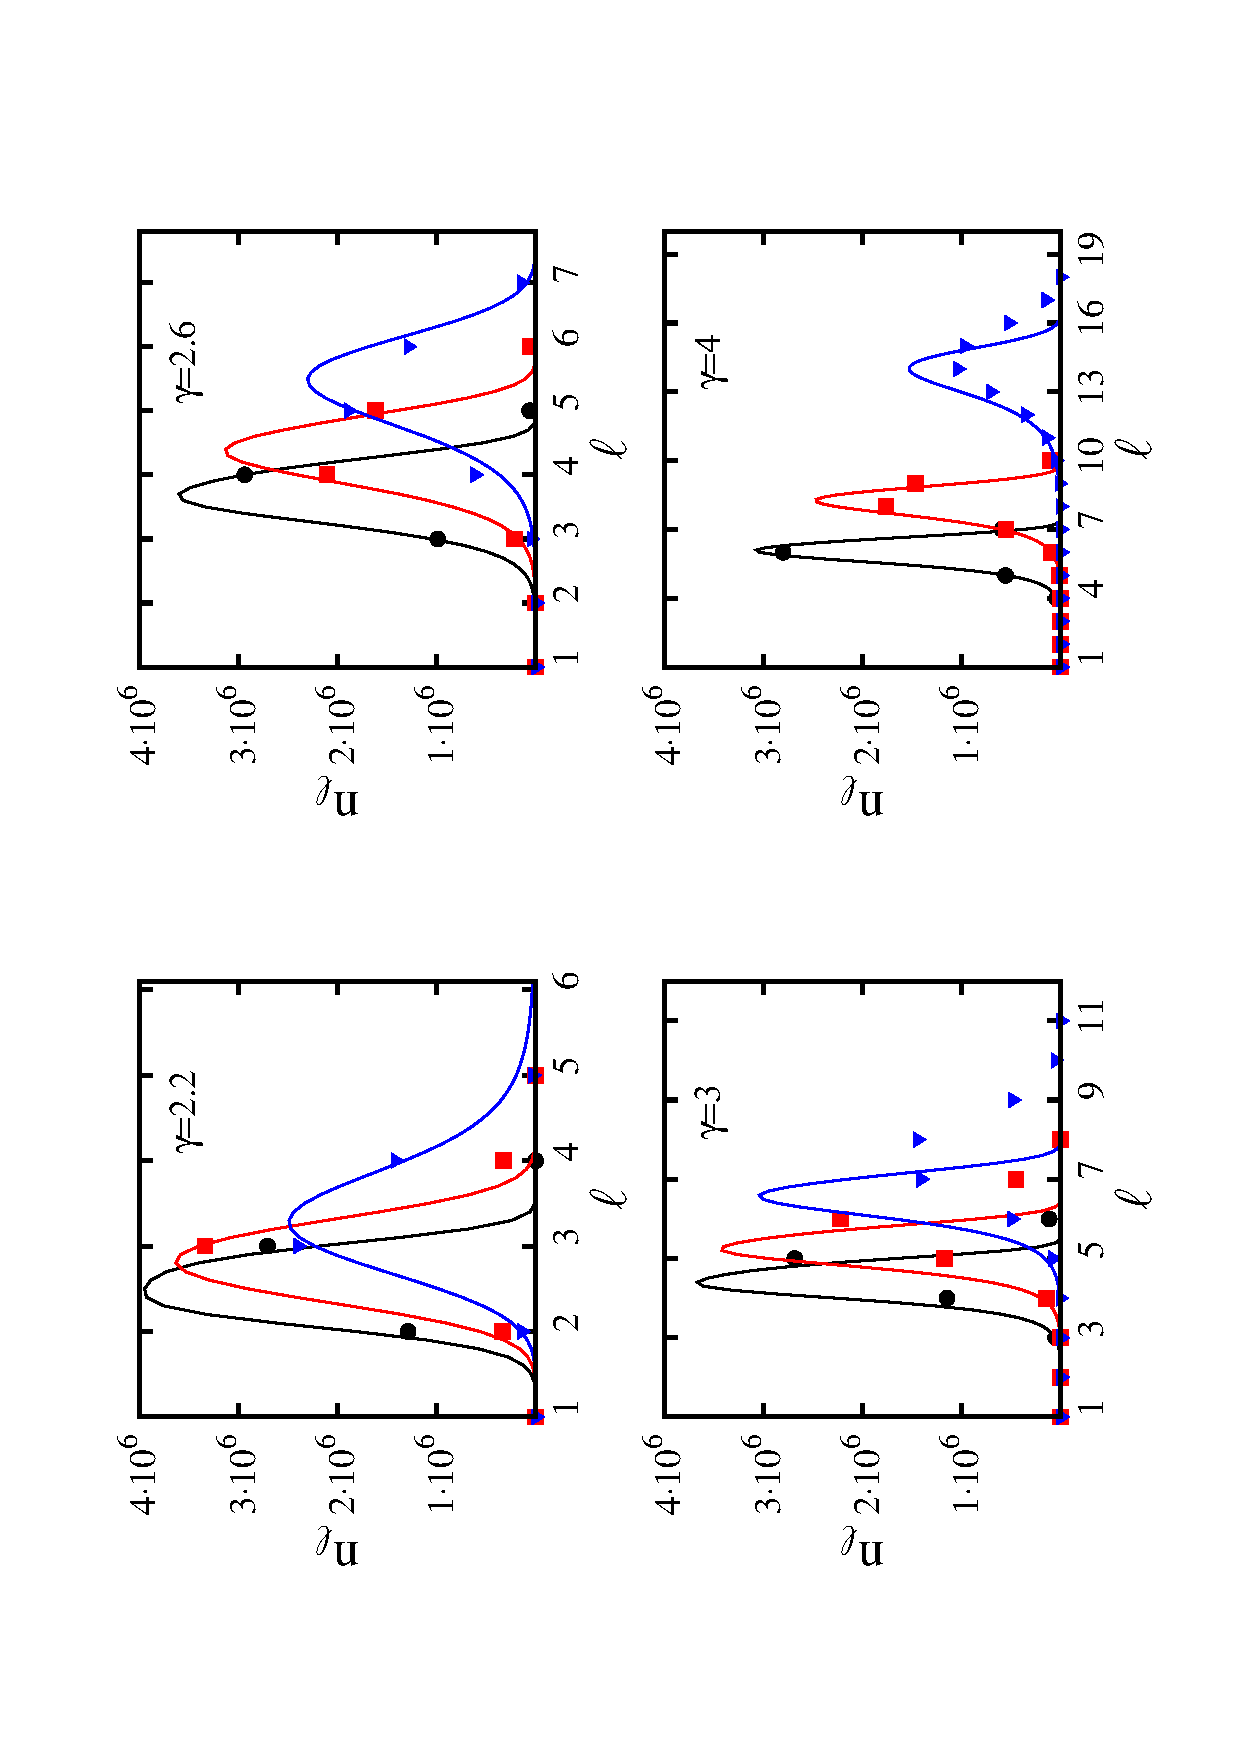
\includegraphics[angle=-90,scale=0.65]{./figures/fig2-3}
	\caption{Nombre de nœuds dans chaque couche pour différentes valeurs de $ \gamma $. Les lignes continues correspondent aux Eq.~\eqref {eq8} et Eq.~\eqref{eq10}. Les symboles sont les simulations numériques d'un réseau de taille $n=4\times10^6$.  Chaque point est la moyenne sur $200$ réalisations. Les couleurs noir, rouge et bleu représentent respectivement les cas $ m = 8, 4 $ et $ 2 $.}
	\label{fig2-3}
\end{figure}

Le cas $\gamma=3$ est le plus problématique. C'est le point où la structure du réseau change radicalement, on passe de la présence de multiples grands hubs et un second moment  $\textless k^2 \textgreater$ qui diverge pour $\gamma<3$, à l'absence de hubs importants et un $\textless k^2  \textgreater$ fini pour $\gamma>3$.
Dans notre approche, le problème se pose lors du calcul de $\sum_{j=1}^{l}p_jn_j$. Néanmoins, en ce point de la transition ($\gamma=3$), certaines propriétés du réseau se comportent presque comme celles pour $\gamma>3$.
Principalement, le plus court chemin est de l'ordre de  $\frac {\ln(n)}{\ln(\ln(n))}$ \cite{Bollobas-Riordan2004}, et $\textless k^2  \textgreater$ reste fini. Nous  utilisons, donc, l'Eq.~\eqref{eq10} pour calculer \nl dans ce cas. \\
Dans la Fig.~\ref{fig2-3}, nous représentons \nl en fonction de $\ell$ pour différentes valeurs de $\gamma$ et $m$. En général, un excellent accord entre la théorie et les simulations est observé. Pour $\gamma=3$, l'accord est moins bon, principalement due au fait que le réseau est encore hétérogène et que les hubs sont toujours présents, alors que nous avons supposé l'homogénéité du réseau pour calculer $\sum_{j=1}^{l} p_jn_j$ dans l'Eq.~\eqref{eq9}. Nous observons aussi une légère  différence  entre la théorie et les simulations lorsque $\gamma=4$ et $m=2$. Ceci est à cause de l'augmentation relative de la proportion de cycles dans les mêmes couches. Ainsi, la structure arborescente parfaite, qui est l'hypothèse principale dans le calcul de \nl, n'est pas très vérifiée. La Fig.~\ref{fig3-3} montre clairement l'importance relative des cycles pour les petites valeurs de $m$. Cet effet est accentué au fur et à mesure qu'on augmente $\gamma$.\\
\begin{figure}[h]
	\begin{center}
		\includegraphics[angle=-90,scale=0.5]{./figures/fig3-3}
	\end{center}
	%\vspace{-10mm}
	\caption{Proportion de cycles dans les couches par rapport à $ m $. De haut en bas, $ \gamma $ est respectivement $ 4, 3, 2.6 $ et $ 2.2 $. Nombre de nœuds $ n = 4.10^6 $, le nombre de réalisations pour chaque point est $200 $.}
	\label{fig3-3}
\end{figure}
Nous observons (Fig.~\ref{fig2-3}) que \nl possède deux allures différentes lors de la croissance et de la décroissance. Pour extraire une information quantitative, concernant les queues de \nl, à partir des Eq.~\eqref{eq8} et Eq.~\eqref {eq10}, on utilise la règle du point milieu. \\
Pour $n$ grand, lorsque $2\textless \gamma \textless 3$, l'Eq.~\eqref{eq8} pour $\ell>1$ peut être approximée comme:
\begin{align}
n_{\ell}&=n\Big(e^{-\frac{\km}{n}\kappa_1^{\frac{1-\beta^{\ell-2}}{1-\beta}}}-e^{-\frac{\km}{n}\kappa_1^{\frac{1-\beta^{\ell-1}}{1-\beta}}}\Big) \nonumber \\
&\approx -n \frac{\partial \Big(e^{-\frac{\km}{n}\kappa_1^{\frac{1-\beta^{\ell-\frac{3}{2}}}{1-\beta}}} \Big) }{\partial \ell} \nonumber \\
&\approx -\frac {\km \ln(\kappa_1) \ln(\beta)} {1-\beta} \beta^{\ell-\frac{3}{2}} \kappa_1^{\frac{1-\beta^{\ell-\frac{3}{2}}}{1-\beta}}e^{-\frac{\km}{n}\kappa_1^{\frac{1-\beta^{\ell-\frac{3}{2}}}{1-\beta}}}, 
\label{eq11}
\end{align}
où $ \ell-\frac{3}{2} $ est utilisé à la place de $ \ell-1$ pour améliorer la différenciation avec la règle du point milieu. Quand $\kappa_1^{\frac{1-\beta^{\ell-\frac{3}{2}}}{1-\beta}}\ll\frac{n}{\km}$,  $e^{-\frac{\km}{n}\kappa_1^{\frac{1-\beta^{\ell-\frac{3}{2}}}{1-\beta}}}\approx 1$, le terme dominant dans l'Eq.~\eqref{eq11}, $\kappa_1^{\frac{1-\beta^{\ell-\frac{3}{2}}}{1-\beta}}$, peut s'écrire comme $\kappa_1^{\frac{1}{1-\beta}}e^{\frac{-e^{\ln(\kappa_1)(\ell-\frac{3}{2})\ln(\beta)}}{1-\beta}}$. Ce dernier terme montre que \nl croit comme une double exponentielle. Après avoir atteint son maximum en $\kappa_1^{\frac{1-\beta^{\ell-\frac{3}{2}}}{1-\beta}}=\frac{n}{\langle k \rangle}$, le terme dominant dans l'Eq.~\ref{eq11} devient 
$e^{-\frac{\langle k \rangle}{n}\kappa_1^{\frac{1-\beta^{\ell-\frac{3}{2}}}{1-\beta}}}$. Pour $\kappa_1^{\frac{1-\beta^{\ell-\frac{3}{2}}}{1-\beta}}\gg \frac{n}{\langle k \rangle}$, \nl décroît comme une triple exponentielle. \\
De la même manière, dans le cas où $\gamma>3$, l'Eq.~\eqref{eq10} peut s'écrire comme
\begin{align}
n_{\ell}&= n(e^{-\frac{\textless k \textgreater}{n}\kappa'\frac{1-\kappa'^{\ell-2}}{1-\kappa'}}-e^{-\frac{\km}{n}\kappa'\frac{1-\kappa'^{\ell-1}}{1-\kappa'}})\nonumber\\
&\approx n\big(e^{-\frac{\km}{n}\kappa'^{\ell-2}}-e^{-\frac{\km}{n}\kappa'^{\ell-1}}\big)\nonumber\\
&\approx n\frac{\partial e^{-\frac{\km}{n}\kappa'^{\ell-\frac{3}{2}}}}{\partial \ell}\nonumber\\
&\approx\km\ln(\kappa')\kappa'^{\ell-\frac{3}{2}}e^{-\frac{\km}{n}\kappa'^{\ell-\frac{3}{2}}},
\end{align}
En suivant les mêmes démarches que précédemment, on obtient une croissance exponentielle pour \nl lorsque $\kappa'^{\ell-\frac{3}{2}} \ll \frac{n}{\km}$ , et une décroissance en double exponentielle lorsque $\kappa'^{\ell-\frac{3}{2}} \gg \frac{n}{\km}$.\\
Nos résultats montrent que \nl décroît toujours plus rapidement qu'elle croit, ceci a été signalé dans le cas du réseau Internet dans \cite{Kalisky-al2006}.\\
Nos résultats analytiques sont aussi comparés aux réseaux du monde réel (voir Fig.~\ref{couch-reel}). La Fig.~\ref{couch-reel} confirme le bon accord  entre nos équations et le réseau Hollywoodien de $392732$ acteurs.  

\begin{figure}[h!]
	\centering
	\includegraphics[scale=0.4,angle=-90]{./figures/bacon}
	\caption{Comparaison entre les données empiriques (cercle) et notre théorie (ligne continue): Les cercles représentent les couches du réseau d’acteurs Hollywoodien de $392732$ acteurs avec $\gamma=2.17$. L'acteur Kevin Bacon est au centre du réseau. La ligne continue représente l'Eq.~\eqref{eq8} avec les mêmes valeurs pour $\gamma$ et $n$. Les résultats empiriques ont été extraits du site: "http://oracleofbacon.org/center.php".}	
	\label{couch-reel}
\end{figure}
    
\section{Plus court chemin}
Le plus court chemin, qu'on désignera par $\textless \ell \textgreater$, est peut être le concept le plus intrigant des réseaux complexes, et ce après la célèbre expérience de Milgram \cite{Mi1967}. Dans cette expérience, Milgram a clairement montré l'effet de petit monde dans les réseaux sociaux, ce qui signifie que deux personnes dans le monde, a priori sans aucun lien, sont séparées en moyenne par un nombre petit de  connexions intermédiaires.\\
De nombreux efforts théoriques ont été déployés pour calculer $\textless \ell\textgreater$ \cite{Chung-Lu2002,Do-al2003,Cohen-Havlin2003,Bollobas-Riordan2004,Fronczak-al2004,Chen-al2018,Melnik-Gleeson}, la plupart d’entre eux se sont focalisés sur la manière dont $\textless \ell \textgreater$ varie avec le nombre de nœuds $n$. Dans le Tableau.~\ref{tab1} on résume les principaux résultats dans la littérature.\\
Une expression analytique de la distance moyenne intégrant les paramètres pertinents du réseau est cruciale pour calculer les centralités d'intermédiarité et de proximité, et peut également présenter un grand intérêt pour des situations réelles. Dans le réseau urbain, par exemple, il a été observé que le trafic des véhicules empruntant les voies de communication les plus courtes est celui de la communicabilité \cite{Akbarzadeh-Estrada2018}.\\
Calculer la distance moyenne dans des réseaux complexes est généralement une tâche ardue. Ici, on déduit $\textless \ell \textgreater$ dans un réseau sans échelle non corrélé à partir de la distribution des nœuds, \nl. En fait, la forme quasi symétrique de \nl sur la Fig.~\ref{fig2-3} suggère que $\textless \ell \textgreater$  correspond à la distance où \nl est maximum, ou également, à la distance où $\frac{\partial n_{\ell}}{\partial\ell}=0$.\\ 
\begin{table}[h]
\center
\begin{tabular}{|c|c|c|}
\hline
Valeur de $\gamma$ & Ordre de grandeur & Désignation \\
\hline
$2<\gamma<3$ & $\sim lnln(n)$& ultra-petit monde \cite{Cohen-Havlin2003,Do-al2003,Cohen-al2002,Chung-Lu2002,Fox-Bellwood2014,Hofstad-al2014}\\
\hline
$\gamma=3$ &$\sim \frac{ln(n)}{lnln(n)}$ & petit monde  \cite{Bollobas1985,Chung-Lu2002,Fronczak-al2004,Hofstad-al2004,Cohen-Havlin2009}\\
\hline
$\gamma>3$ &$\sim ln(n)$& petit monde \cite{Bollobas1985,Chung-Lu2002,Fronczak-al2004,Hofstad-al2004,Cohen-Havlin2009}\\
\hline
\end{tabular}
\caption{Principaux résultats sur le plus court chemin en fonction de $\gamma$.}
\label{tab1}
\end{table}
Nous commençons par le cas le plus simple $\gamma=2$. Comme déjà mentionné, il y a un maximum de deux couches dans le réseau, $\textless \ell \textgreater$  s'écrit comme:
   \begin{align}
   	\textless \ell \textgreater=\frac{\km+2(n-\km)}{n},
   	\label{eq14}  
   \end{align}
qui tend vers $2$ pour un grand $n$. Cela signifie que presque tous les nœuds sont connectés entre eux à travers le nœud de degré maximum. \\
Quand $ 2<\gamma<3 $, aucune solution pour $\frac{\partial n_{\ell}}{\partial\ell}=0$ ne peut être trouvée directement à partir de l'Eq.~\eqref{eq8}, alors nous utilisons l'approximation donnée dans l'Eq.~\eqref{eq11}, où \nl est maximum quand $\kappa_1^{\frac{1-\beta^{\textless \ell \textgreater-\frac{3}{2}}}{1-\beta}}=\frac{n}{\km}$. Après avoir remplacé $\kappa_1 $ et $K_1$ par leurs expressions correspondantes, on obtient:
\begin{align}
	\textless \ell \textgreater=\frac{\ln\big(1-\frac{\ln(n)-\ln(\km)}{\ln(n)+\frac{\gamma-1}{3-\gamma}\ln(\frac{\gamma-2}{3-\gamma}m)}\big)}{\ln\big(\frac{2\gamma-4}{\gamma-1}\big)}+\frac{3}{2}.
	\label{eq12}
\end{align}
pour $n$ grand, $\textless \ell \textgreater \approx -\frac{\ln(\ln(n))}{\ln(\beta)}$.
Cette forme d'échelle est derrière la désignation ultra-petit monde \cite{Cohen-Havlin2003}, et elle est largement acceptée pour cet intervalle de $\gamma $ \cite{Do-al2003,Cohen-al2002,Chung-Lu2002,Fox-Bellwood2014,Hofstad-al2014}.\\
Pour $\gamma\ge 3 $, $\textless \ell \textgreater$ peut être déduit de l'Eq.~\eqref{eq10} en résolvant $\frac{\partial n_{\ell}}{\partial\ell}=0$. Cela donne:
\begin{align}
	\textless \ell \textgreater=\frac{\ln (n)}{\ln(\kappa')}+\frac{\ln(\ln(\kappa'))-\ln(\km)}{\ln(\kappa')}+1.
	\label{eq13}
\end{align}
Si $\gamma>3$, $\kappa$ est constant (Eq.~\eqref{eq4}). Pour un grand $n$, $\textless\ell\textgreater\approx\frac{\ln(n)} {\ln(\kappa')}$, qui est la forme d'échelle rapportée dans de nombreux autres travaux \cite{Bollobas1985,Chung-Lu2002,Fronczak-al2004,Hofstad-al2004,Cohen-Havlin2009}, et connu comme l'effet de petit monde. \\
 \begin{figure}[h]
 	\centering
 	\includegraphics[scale=1.3]{./figures/fig4-3}
 	\caption{Le plus court chemin en fonction du nombre de nœuds. Les valeurs de $\gamma$ de haut en bas sont respectivement $ 4, 3, 2.6 $ et $ 2.2 $. Les lignes continues correspondent à l'Eq.~\eqref{eq12} et à l'Eq.~\eqref{eq13}. Les lignes discontinues correspondent aux équations dans \cite{Fronczak-al2004}. Chaque simulation est moyennée sur plus de $200$ réalisations.}
 	\label{fig4-3}
 \end{figure}
Quand $\gamma=3$, $\kappa$ dépend de $K$, qui dépend à son tour de $n$. Prenant $\kappa_1=m(\ln(K)-\ln(m))$ et $K=mn^{\frac{1}{\gamma-1}}$, nous trouvons pour  $n$ grand, $\textless\ell\textgreater\approx \frac{\ln(n)} {\ln(\ln(n))} $. Ce résultat est en accord avec les travaux précédents \cite {Chung-Lu2002,Cohen-Havlin2003,Fronczak-al2004,Bollobas-Riodan2002}, et confirme le cas particulier de $ \gamma = 3 $. En effet, la présence des hubs rend les distances entre les nœuds plus petites que celles où les hubs sont absents ($\gamma>3$), en même temps les hubs ne sont pas suffisamment grands pour faire des distances ultra-petites comme lorsque $2<\gamma<3$.\\  
Comme nous avons signalé dans la Section.~\ref{PCC}, les travaux importants \cite{Do-al2003,Cohen-Havlin2003} dans ce sujet donnent seulement l'allure de $\textless \ell \textgreater$  pour les grandes valeurs de $n$. L'exception est la contribution de Fronczak et  al. \cite{Fronczak-al2004} où ils ont trouvé des équations fermées en fonction des paramètres du réseau, ces équations prédisent que $\textless \ell \textgreater$  tend vers une valeur constante lorsque $n$ tend vers l'infini pour $2<\gamma<3$, ce qui est en contradiction avec les principaux résultats dans la littérature  \cite{Cohen-Havlin2003,Do-al2003,Cohen-al2002,Chung-Lu2002,Fox-Bellwood2014,Hofstad-al2014}, et avec la simulation numérique (voir Fig.~\ref{fig4-3}).\\ Nos résultats (Fig.~\ref{fig4-3}) montrent un très bon accord avec les simulations pour $\gamma\neq3$. Pour $\gamma=3$,  notre approche donnent des valeurs de $\textless \ell \textgreater$ relativement proches des simulations numériques, et ils sont également très similaires aux résultats de \cite{Fronczak-al2004}.
 \section{conclusion} 
Dans ce chapitre, nous avons étudié en détail certains aspects fondamentaux des réseaux sans échelle non corrélés. \`{A} partir d'arguments probabilistes, nous avons obtenu des expressions explicites, en fonction de l'exposant de degré $\gamma$, pour le nombre de nœuds, \nl, à une distance donnée d'un nœud arbitraire. Nous avons montré que le réseau hétérogène ($2 \textless \gamma \textless 3$) peut être
approximé par un réseau sans échelle ordonné où les nœuds voisins du nœud racine (choisi aléatoirement) sont placés du plus grand au plus petit degré. Ceci peut simplifier les calculs, qui sont en général assez difficiles, dans plusieurs situations des réseaux hétérogènes.\\
Nous avons aussi décrit avec précision les formes des queues de la distribution \nl.\\
Profitant de la forme de celle-ci, nous avons pu déduire les expressions explicites du plus court chemin pour différentes valeurs de $\gamma$. Les expressions obtenues reproduisent les comportements asymptotiques connues pour $n$ grand, à savoir, l'ultra-petit monde pour $2<\gamma<3$, et le petit monde pour $\gamma\ge 3$. Nos résultats théoriques concordent très bien avec les simulations numériques et le nombre de Bacon, sauf dans le cas $\gamma=3$, où nous avons observé la même forme, comme pour les autres valeurs de $\gamma$, dans les queues de \nl, mais avec une notable différence (entre la théorie et la simulation) dans la position du maximum. Cette différence n'affecte pas l'ordre de grandeur du plus court chemin pour cette valeur de $\gamma$.
\let\cleardoublepage\clearpage
